\chapter{Arhitektura i dizajn sustava}
		
	\vspace{-1cm}
	\begin{figure}[h]
		\begin{center}
			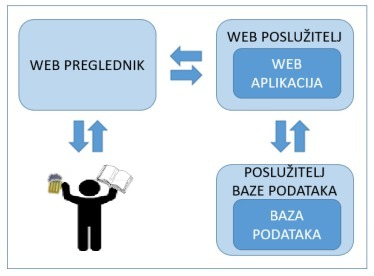
\includegraphics{slike/arhitektura_skica.png}
			\caption{Arhitektura sustava}
		\end{center}	
	\end{figure}
	
	\indent Arhitekturu tvore tri podsustava: web poslužitelj, web aplikacija te baza podataka. \textit{Web preglednik} je program za pregledavanje i navigaciju web-stranicama. Kada korisnik pošalje zahtjev za web-stranicom, preglednik dohvaća potrebne datoteke s \textit{web poslužitelja} i prikazuje stranicu na korisnikovom ekranu u namijenjenom obliku. Poslužitelj omogućuje komunikaciju klijenta s \textit{web aplikacijom} koja je na njemu pokrenuta, a prosljeđuje joj zahtjeve HTTP-om (engl. \textit{Hyper Text Transfer Protocol}). Web aplikacija odgovara na zahtjeve klijenta pristupajući po potrebi bazi podataka i vraćajući HTML dokument čitljiv u web pregledniku. \\
	
	\indent Za izradu ovog projekta koristili smo se Spring Boot frameworkom u Javi kroz razvojno okruženje IntelliJ Community Edition, Javascriptom uz React u Visual Studio Code-u te nizom drugih programa za dizajn slika i grafova (GIMP, AstahUML itd.). \\
	
	\indent Arhitektura sustava prati MVC obrazac, odnosno Model-Pogled-Nadglednik (engl. \textit{Model View Controller}), stilističku varijaciju arhitekture zasnovane na događajima. Takve arhitekture odlikuje to što se komponente međusobno ne pozivaju eksplicitno, već neke od njih generiraju signale (događaje) ne znajući koja druga "osluškuje" tj. očekuje takav signal i na njega reagira. Kod MVC-a pogodno je što smanjuje međuovisnost korisničkog sučelja i ostatka sustava, a omogućuje i nezavisan razvoj, nadogradnje i dodavanje različitih dijelova aplikacije. Sadrži različite gotove predloške za klase koji nam olakšavaju proces izrade.\\
	
	\indent MVC model sastoji se od komponenti:
	\begin{packed_item}
		\item 	\textbf{Model} - Središnja komponenta sustava, sadrži razrede čiji se objekti obrađuju. Rukuje s podatkovnom logikom i bazom podataka. Prima podatke od nadglednika.
		\item 	\textbf{Pogled} - Predstavlja model korisniku na čitljiv način. Sadrži razrede čiji objekti služe za prikaz podataka. Dinamički se osvježava.
		\item	\textbf{Nadglednik} - Razumije naputke korisnika i pretvara ih u upute ka modelu. Sadrži razrede koji upravljaju i rukuju korisničkom interakcijom s pogledom i modelom, poput poslovne logike i odgovora na događaje.
	\end{packed_item}

	\eject
		

		

				
		\section{Baza podataka}
			

		
		Za potrebe našeg sustava koristit ćemo relacijsku bazu podataka koja svojom strukturom olakšava modeliranje stvarnog svijeta. Gradivna jedinka baze je relacija, odnosno tablica koja je definirana svojim imenom i skupom atributa. Zadaća baze podataka je brza i jednostavna pohrana, izmjena i dohvat podataka za daljnju obradu. Baza podataka ove aplikacije sastoji se od sljedećih entiteta:
		
		\begin{itemize}
			\item Korisnik
			\item Uloga
			\item Vrsta
			\item Oznaka
			\item ImaUlogu
			\item JePrijatelj
			\item JeBlokiranOd
			\item Dogadjaj
			\item Pohadja
			\item ImaOznaku
			
		\end{itemize}
		
		
			\subsection{Opis tablica}
			

				
				
				\noindent\textbf{Korisnik} Ovaj entitet sadržava sve važne informacije o korisniku aplikacije. Sadrži atribute: id korisnika, nadimak, korisničko ime, email, salt, lozinka i suspendiran. Ovaj entitet u vezi je Many-to-Many s Uloga preko veze imaUlogu, u vezi Many-to-Many s Korisnik preko veze jePrijatelj, u vezi Many-to-Many s Korisnik preko veze JeBlokiranOd, te u vezi  One-to-Many s entitetom Događaj preko i u vezi Many-to-Many s entitetom Dogadjaj preko veze Pohadja.
				
				\begin{longtblr}[
					label=none,
					entry=none
					]{
						width = \textwidth,
						colspec={|X[6,l]|X[6, l]|X[20, l]|}, 
						rowhead = 1,
					} %definicija širine tablice, širine stupaca, poravnanje i broja redaka naslova tablice
					\hline \multicolumn{3}{|c|}{\textbf{Korisnik}} & tip podataka & opis varijable	 \\ \hline[3pt]
					\SetCell{LightGreen}id korisnik & BIGINT NOT NULL	&  	jedinstveni brojčani identifikator korisnika	\\ \hline
					nadimak	& VARCHAR(25) NOT NULL &   nadimak korisnika	\\ \hline
					korisnicko ime & VARCHAR(25) NOT NULL & ime korisnika  \\ \hline  
					email & VARCHAR(255) NOT NULL & email korisnika  \\ \hline 
					salt & BYTEA NOT NULL	&  salt za hashiranje lozinke		\\ \hline 
					lozinka & BYTEA NOT NULL	&  	hash lozinke	\\ \hline 
					suspendiran & BOOLEAN NOT NULL	& oznaka je li korisnik suspendiran 		\\ \hline 
					
				\end{longtblr}
			
			
				\noindent\textbf{Uloga} Ovaj entitet sadržava sve važne informacije o ulogama korisnika. Sadrži atribute: id uloga, naziv uloga i opis uloga. Ovaj entitet u vezi je Many-to-Many s Korisnik preko veze imaUlogu.
				
				\begin{longtblr}[
					label=none,
					entry=none
					]{
						width = \textwidth,
						colspec={|X[6,l]|X[6, l]|X[20, l]|}, 
						rowhead = 1,
					} %definicija širine tablice, širine stupaca, poravnanje i broja redaka naslova tablice
					\hline \multicolumn{3}{|c|}{\textbf{Uloga}}& tip podataka & opis varijable	 \\ \hline[3pt]
					\SetCell{LightGreen}id uloga & BIGINT NOT NULL	&  	jedinstveni brojčani identifikator uloge korisnika	\\ \hline
					naziv uloga	& VARCHAR(255) NOT NULL &  naziv uloge korisnika	\\ \hline 
					opis uloga & VARCHAR(255) NOT NULL & opis uloge korisnika  \\ \hline 
					
				\end{longtblr}
			
				\noindent\textbf{Vrsta} Ovaj entitet sadržava sve važne informacije o vrstama događaja. Sadrži atribute: id vrsta, naziv vrsta i opis vrsta. Ovaj entitet u vezi je Many-to-On s entitetom Dogadjaj preko identifikatora vrste u entitetu Dogadjaj.
				
				\begin{longtblr}[
					label=none,
					entry=none
					]{
						width = \textwidth,
						colspec={|X[6,l]|X[6, l]|X[20, l]|}, 
						rowhead = 1,
					} %definicija širine tablice, širine stupaca, poravnanje i broja redaka naslova tablice
					\hline \multicolumn{3}{|c|}{\textbf{Vrsta}}& tip podataka & opis varijable	 \\ \hline[3pt]
					\SetCell{LightGreen}id vrsta & INT NOT NULL	&  jedinstveni brojčani identifikator vrste događaja	\\ \hline
					naziv vrsta	& VARCHAR(255) NOT NULL &  naziv vrste događaja	\\ \hline 
					opis vrsta & VARCHAR(255) NOT NULL &  opis vrste događaja \\ \hline 
					 
				\end{longtblr}
				
				\noindent\textbf{Oznaka} Ovaj entitet sadržava sve važne informacije o oznakama događaja. Sadrži atribute: id oznaka, naziv oznaka i boja hex. Ovaj entitet u vezi je Many-to-Many s Oznaka preko veze imaOznaku.
				
				\begin{longtblr}[
					label=none,
					entry=none
					]{
						width = \textwidth,
						colspec={|X[6,l]|X[6, l]|X[20, l]|}, 
						rowhead = 1,
					} %definicija širine tablice, širine stupaca, poravnanje i broja redaka naslova tablice
					\hline \multicolumn{3}{|c|}{\textbf{Oznaka}}& tip podataka & opis varijable	 \\ \hline[3pt]
					\SetCell{LightGreen}id oznaka & INT NOT NULL	& jedinstveni brojčani identifikator oznake događaja	\\ \hline
					naziv oznaka	& VARCHAR(255) NOT NULL &  naziv oznake događaja  	\\ \hline 
					boja hex & CHAR(7) NOT NULL & boja oznake  \\ \hline 
					
				\end{longtblr}
				
				
				\noindent\textbf{ImaUlogu} Ova veza sadržava sve važne informacije po kojima saznajemo koji korisnik ima koju ulogu. Sadrži atribute: id korisnik i id uloga. Povezuje entitete Korisnik i Uloga. 
				
				\begin{longtblr}[
					label=none,
					entry=none
					]{
						width = \textwidth,
						colspec={|X[6,l]|X[6, l]|X[20, l]|}, 
						rowhead = 1,
					} %definicija širine tablice, širine stupaca, poravnanje i broja redaka naslova tablice
					\hline \multicolumn{3}{|c|}{\textbf{ImaUlogu}}& tip podataka & opis varijable	 \\ \hline[3pt]
					\SetCell{LightGreen}id korisnik & BIGINT NOT NULL	&  	jedinstveni brojčani identifikator korisnika (korisnik.id korisnik)	\\ \hline
					\SetCell{LightGreen}id uloga	& BIGINT NOT NULL &   jedinstveni brojčani identifikator uloga korisnika (uloga.id uloga)	\\ \hline 
					 
				\end{longtblr}
				
				\noindent\textbf{JePrijatelj} Ova veza sadržava sve važne informacije o tome koji je korisnik nekom drugom korisniku prijatelj. Sadrži atribute: id korisnik i id prijatelj. Povezuje entitet Korisnik sa samim sobom.
				
				\begin{longtblr}[
					label=none,
					entry=none
					]{
						width = \textwidth,
						colspec={|X[6,l]|X[6, l]|X[20, l]|}, 
						rowhead = 1,
					} %definicija širine tablice, širine stupaca, poravnanje i broja redaka naslova tablice
					\hline \multicolumn{3}{|c|}{\textbf{JePrijatelj}}	& tip podataka & opis varijable \\ \hline[3pt]
					\SetCell{LightGreen}id korisnik & BIGINT NOT NULL	&  	jedinstveni brojčani identifikator korisnika (korisnik.id korisnik)	\\ \hline
					\SetCell{LightGreen}id prijatelj	& BIGINT NOT NULL	& jedinstveni brojčani identifikator drugog korisnika prijatelja (korisnik.id korisnik)	\\ \hline 
				\end{longtblr}
			
			
				\noindent\textbf{JeBlokiranOd} Ova veza sadržava sve važne informacije o tome koji je korisnik blokiran i od kojeg je korisnika blokiran. Sadrži atribute: id blokiran i id blokiran od. Povezuje entitet Korisnik sa samim sobom.
				
				\begin{longtblr}[
					label=none,
					entry=none
					]{
						width = \textwidth,
						colspec={|X[6,l]|X[6, l]|X[20, l]|}, 
						rowhead = 1,
					} %definicija širine tablice, širine stupaca, poravnanje i broja redaka naslova tablice
					\hline \multicolumn{3}{|c|}{\textbf{JeBlokiranOd}}	& tip podataka & opis varijable \\ \hline[3pt]
					\SetCell{LightGreen}id blokiran & BIGINT NOT NULL	&  	jedinstveni brojčani identifikator korisnika koji je blokiran (korisnik.id korisnik)	\\ \hline
					\SetCell{LightGreen}id blokiran od	& BIGINT NOT NULL &   jedinstveni brojčani identifikator korisnika koji blokira (korisnik.id korisnik)	\\ \hline 
				 
				\end{longtblr}
				
				
				\noindent\textbf{Dogadjaj} Ovaj entitet sadržava sve važne informacije o događaju. Sadrži atribute: id događaj, naziv, mjesto, vrijeme početka, vrijeme kraja, opis, promoviran, koordinate, id organizator i id vrsta. Ovaj entitet u vezi je Many-to-One s entitetom Vrsta preko identifikatora vrste, u vezi Many-to-One s entitetom Korisnik preko identifikatora korisnika, u vezi Many-to-Many s entitetom Korisnik preko veze Pohadja i u vezi Many-to-Many s Oznaka preko veze imaOznaku.
				
				\begin{longtblr}[
					label=none,
					entry=none
					]{
						width = \textwidth,
						colspec={|X[6,l]|X[6, l]|X[20, l]|}, 
						rowhead = 1,
					} %definicija širine tablice, širine stupaca, poravnanje i broja redaka naslova tablice
					\hline \multicolumn{3}{|c|}{\textbf{Dogadjaj}}	& tip podataka & opis varijable \\ \hline[3pt]
					\SetCell{LightGreen}id dogadjaj & BIGINT NOT NULL	&  	jedinstveni brojčani identifikator događaja  	\\ \hline
					naziv	& VARCHAR(255) NOT NULL & naziv događaja  	\\ \hline 
					mjesto & VARCHAR(255) NOT NULL & mjesto zbivanja događaja  \\ \hline 
					vrijeme poc & TIMESTAMP NOT NULL	& vrijeme počinjanja događaja 		\\ \hline 
					vrijeme kraj & TIMESTAMP NOT NULL	&  	vrijeme završetka događaja	\\ \hline
					opis & VARCHAR(255) NOT NULL & opis događaja \\ \hline
					promoviran & BOOLEAN NOT NULL &  oznaka je li događaj promoviran \\ \hline 
					koordinate & VARCHAR(255) NOT NULL & koordinate događaja \\ \hline
					\SetCell{LightBlue}id organizator & BIGINT NOT NULL &   jedinstveni brojčani identifikator organizatora događaja (korisnik.id korisnik) \\ \hline 
					\SetCell{LightBlue}id vrsta & INT NOT NULL & jedinstveni brojčani identifikator vrste događaja (vrsta.id vrsta)
					\\ \hline
				\end{longtblr}
				
				
				\noindent\textbf{Pohadja} Ova veza sadržava sve važne informacije o tome tko je pohađao koji događaj i kako ga je ocijenio. Sadrži atribute: recenzija, id polaznika i id događaja. Povezuje entitete Korisnik i Dogadjaj.
				
				\begin{longtblr}[
					label=none,
					entry=none
					]{
						width = \textwidth,
						colspec={|X[6,l]|X[6, l]|X[20, l]|}, 
						rowhead = 1,
					} %definicija širine tablice, širine stupaca, poravnanje i broja redaka naslova tablice
					\hline \multicolumn{3}{|c|}{\textbf{Pohadja}}	& tip podataka & opis varijable \\ \hline[3pt]
					recenzija & SMALLINT NOT NULL	&  recenzija korisnika za događaj	\\ \hline
				    \SetCell{LightGreen} id pohadjatelja	& BIGINT NOT NULL &  jedinstveni brojčani identifikator pohađatelja (korisnik.id korisnik)	\\ \hline 
					\SetCell{LightGreen} id dogadjaja & BIGINT NOT NULL &  jedinstveni brojčani identifikator događaja (dogadjaj.id dogadjaj) \\ \hline 
					 
				\end{longtblr}
			
				
				\noindent\textbf{ImaOznaku} Ovaa veza sadržava sve važne informacije o oznakama određenih događaja. Sadrži atribute: id događaj i id oznaka. Povezuje entitete Oznaka i Dogadajaj.
				
				\begin{longtblr}[
					label=none,
					entry=none
					]{
						width = \textwidth,
						colspec={|X[6,l]|X[6, l]|X[20, l]|}, 
						rowhead = 1,
					} %definicija širine tablice, širine stupaca, poravnanje i broja redaka naslova tablice
					\hline \multicolumn{3}{|c|}{\textbf{ImaOznaku}}	& tip podataka & opis varijable \\ \hline[3pt]
					\SetCell{LightGreen}id dogadjaj & BIGINT NOT NULL	&  	jedinstveni brojčani identifikator događaja (dogadjaj.id dogadjaj)	\\ \hline
					\SetCell{LightGreen}id oznaka	& INT NOT NULL &   jedinstveni brojčani identifikator oznake (oznaka.id oznaka)	\\ \hline 
				
				\end{longtblr}
			
				
			
			
				
				
			
			\subsection{Dijagrami baze podataka}
				
			\begin{figure}[h]
				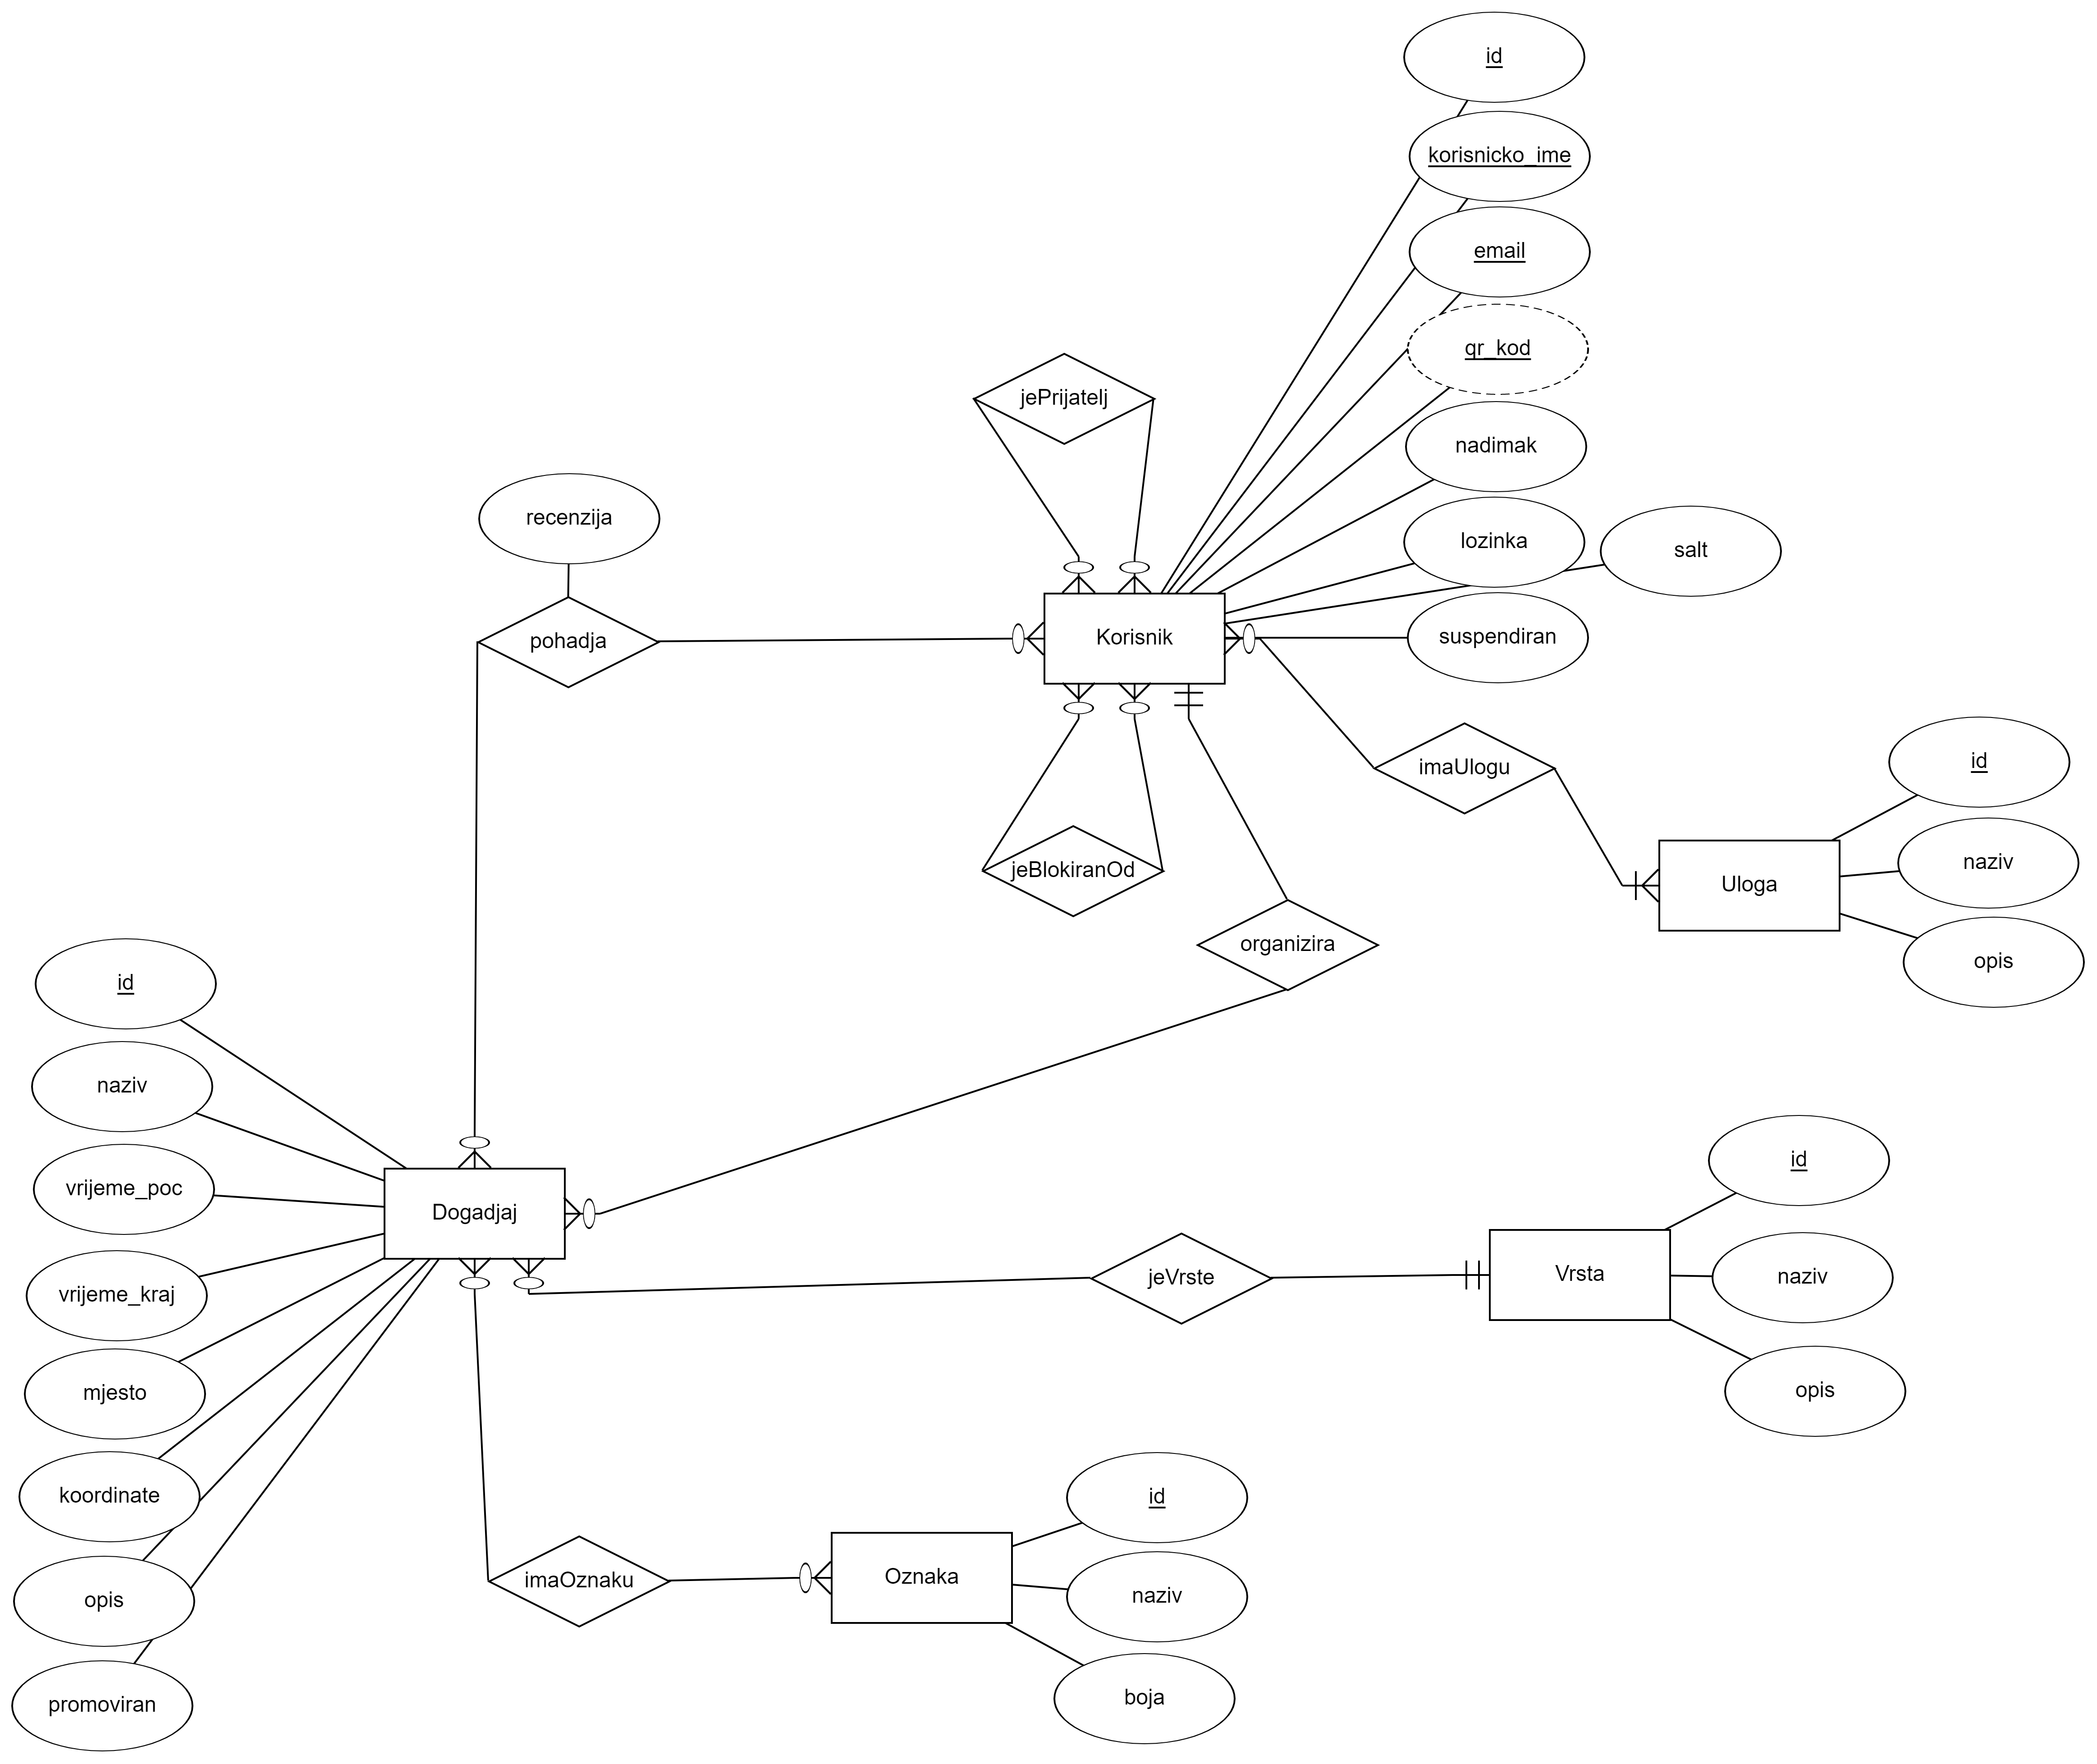
\includegraphics[width=\textwidth]{dijagrami/Baza podataka/ER model.png}
				\caption{ER dijagram baze podataka}
			\end{figure}
				
			\newpage
			\vfill	
			
			\begin{figure}[h]
				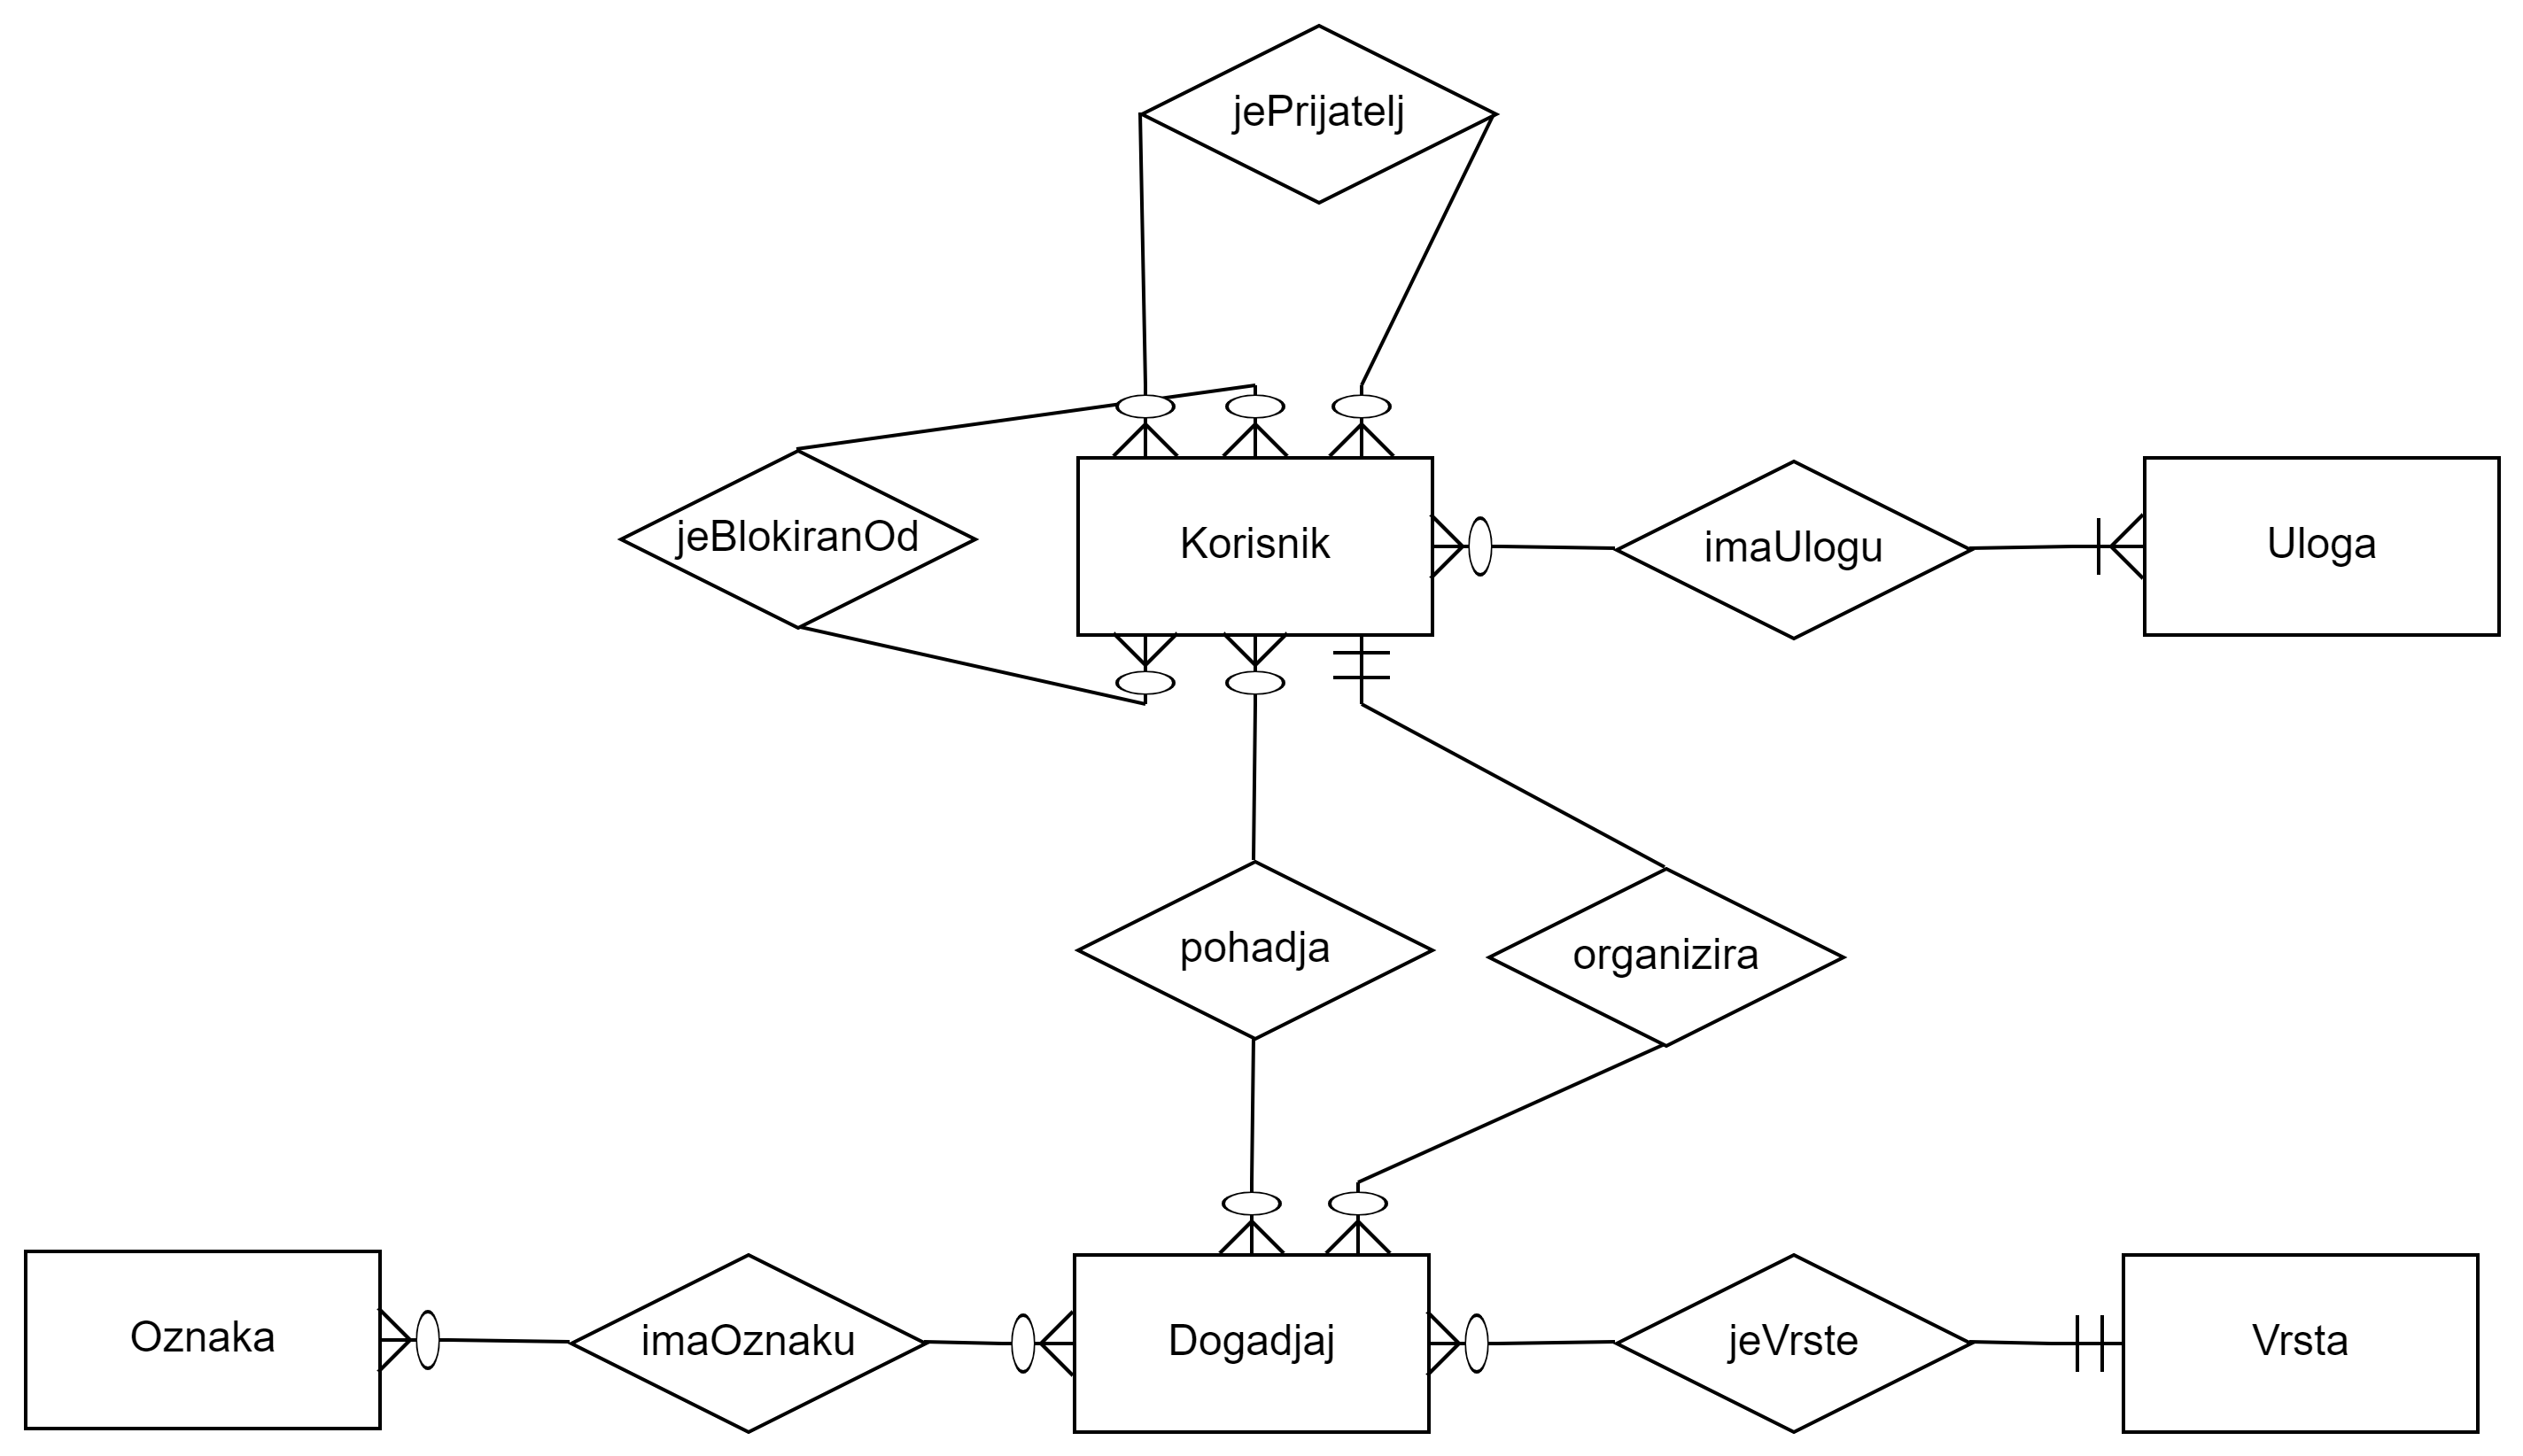
\includegraphics[width=\textwidth]{dijagrami/Baza podataka/ER model (bez atributa).png}
				\caption{ER dijagram baze podataka bez atributa}
			\end{figure}
				
			\begin{figure}[H]
				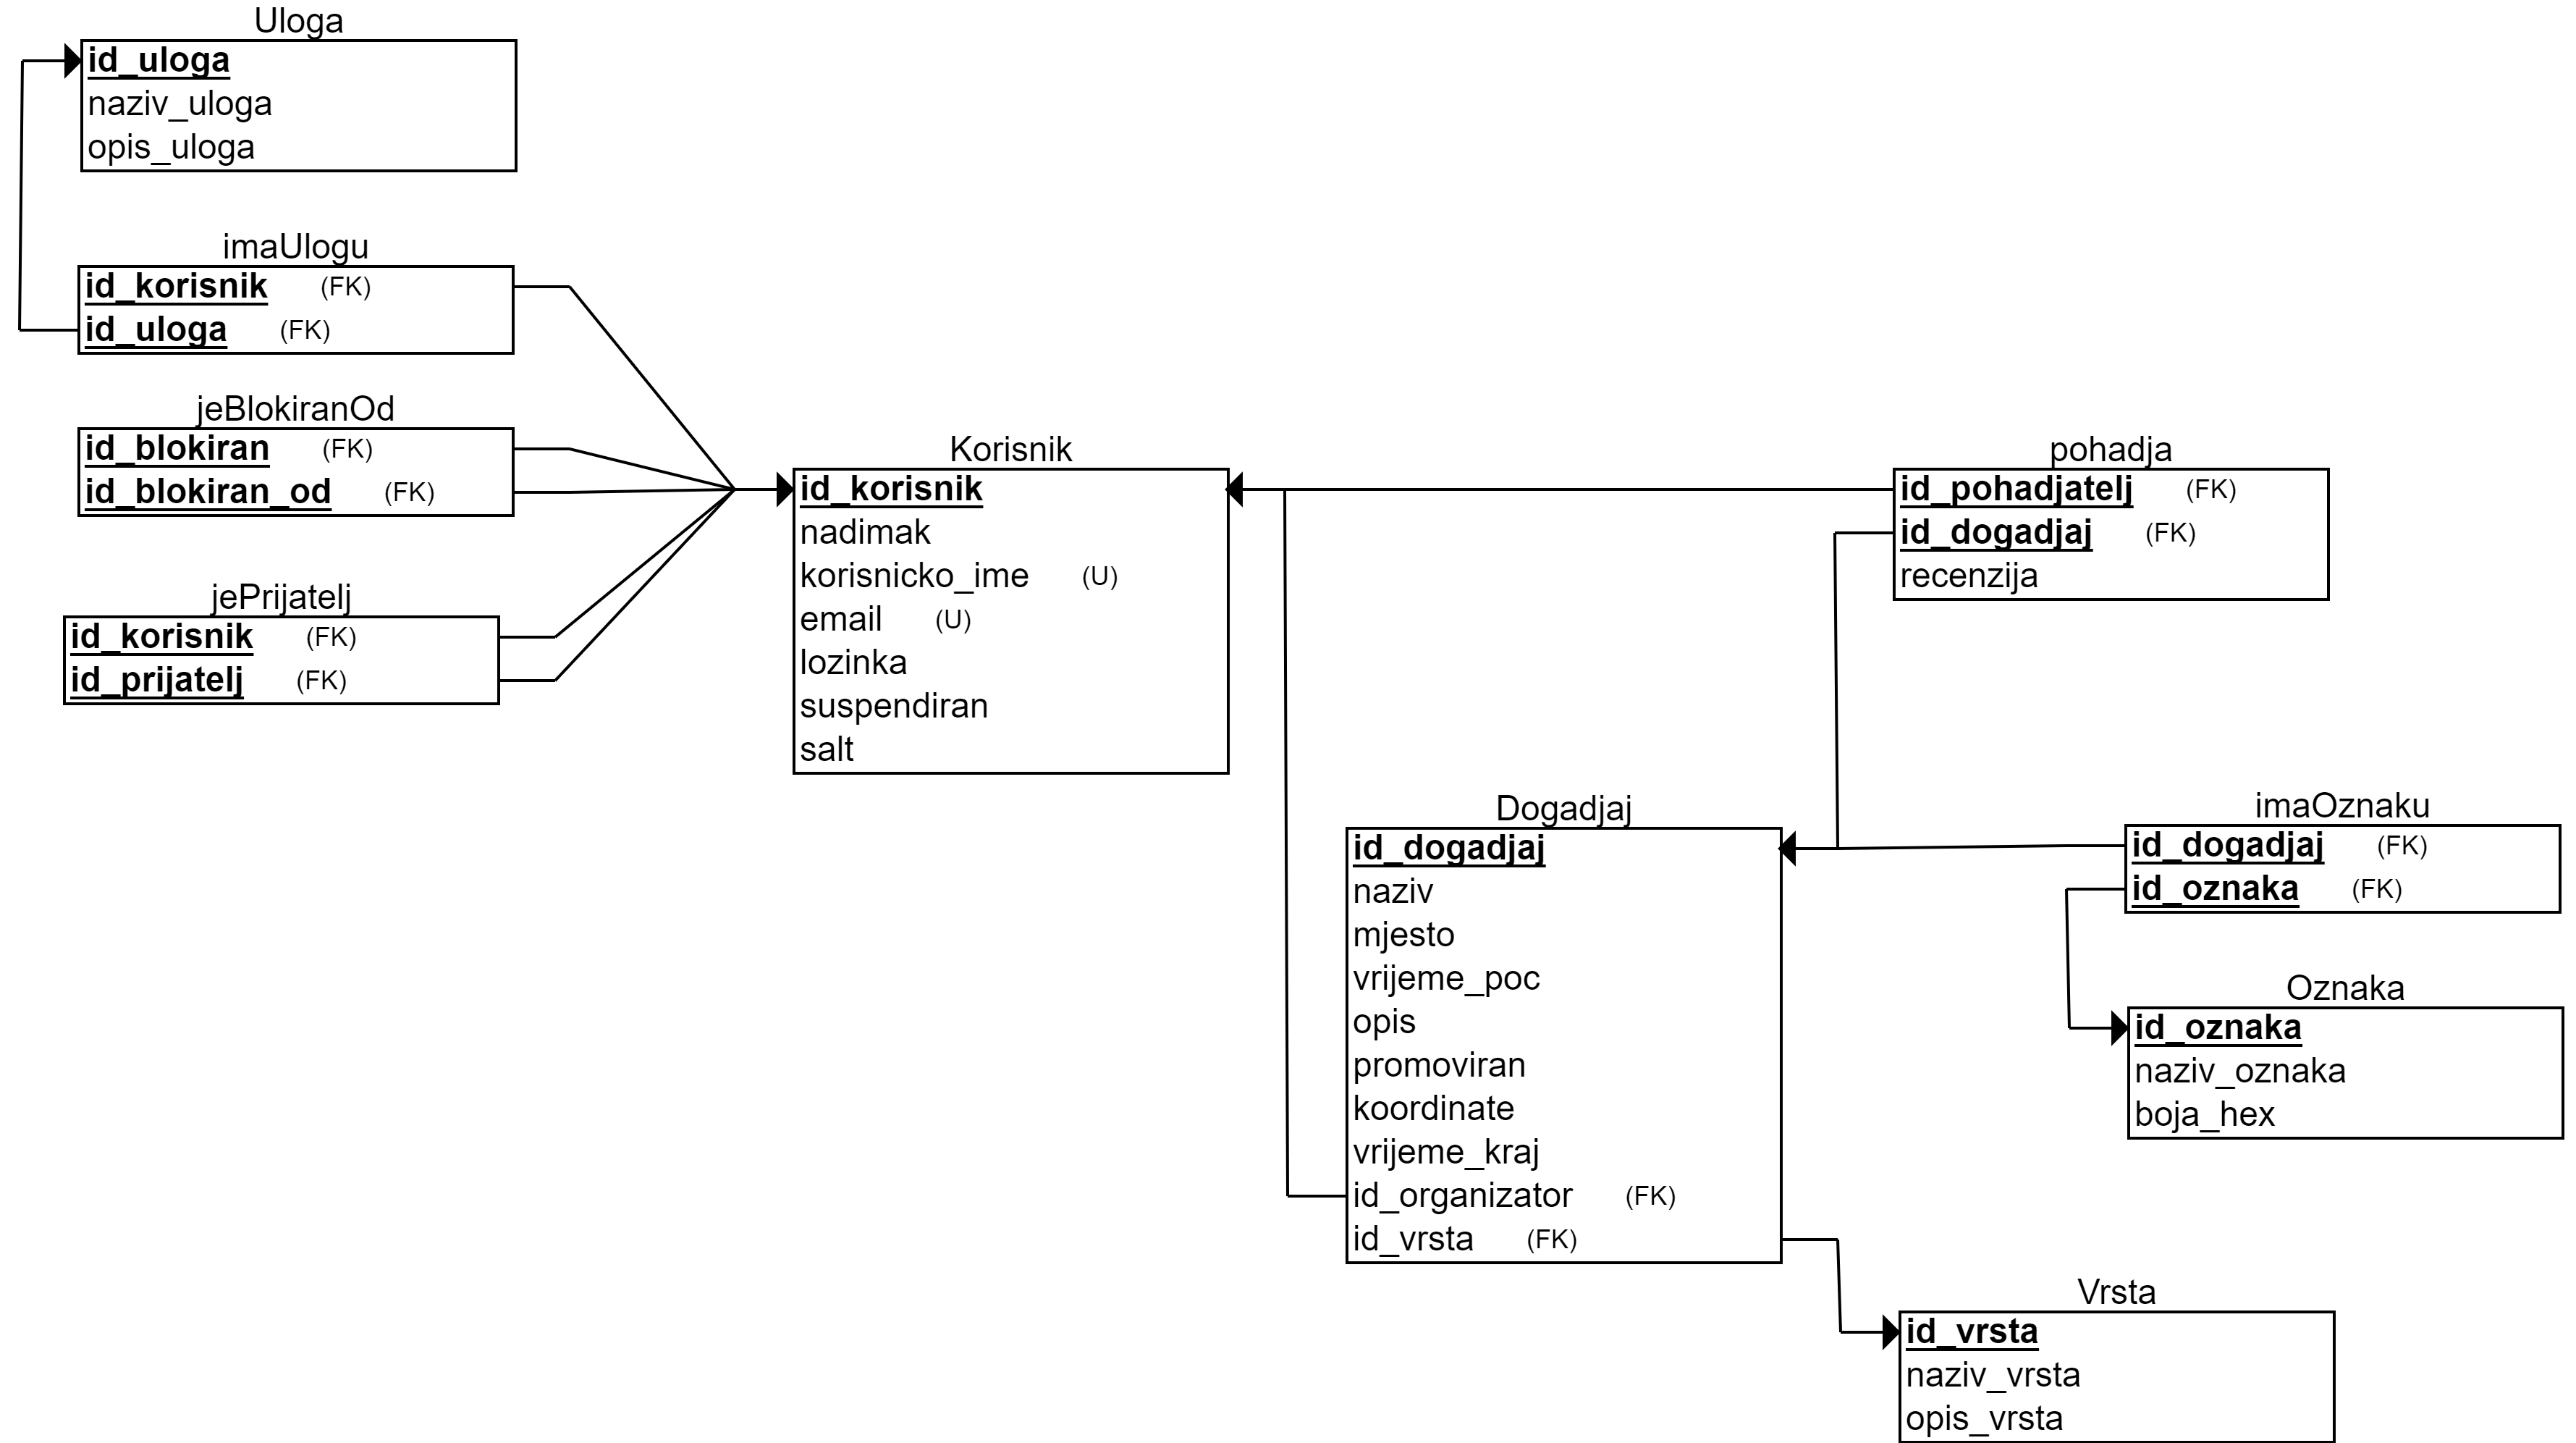
\includegraphics[width=\textwidth]{dijagrami/Baza podataka/REL shema.png}
				\caption{Relacijski dijagram baze podataka}
			\end{figure}
				
			\vfill
			\clearpage
			
			\eject
			
			
		\section{Dijagram razreda}
			
			\indent Na naredne tri slike nalaze se dijagrami razreda podijeljeni logički po srodnosti. Neki razredi povezani su i s onima na odvojenim slikama što se da zaključiti po nazivima njihovih metoda. \\
			
			\indent Razredi na slici 4.6 uokvireni plavom bojom su kontroleri. Njihove metode služe za primanje i slanje DTO-ova (\textit{Data Transfer Objects})  prema frontendu u obliku JSON datoteka s html statusnim kodom. Pozivaju funkcije servisa. Razlikuju se kontroleri za korisnike, događaje te postupke prijave i registracije. Sami DTO razredi nalaze se na slici 4.5, a to su zahtjevi i odgovori za prijavu i registraciju.\\
			
			\indent Razredi na slici 4.6 uokvireni crvenom bojom su servisi. Služe za komunikaciju između repozitorija i kontrolera.\\
			
			\indent Razredi na slici 4.6 uokvireni zelenom bojom su repozitoriji. Služe za pozivanje SQL upita nad bazom podataka.\\
			
			\indent Razredi na slici 4.7 su modeli. Modeliraju potrebne razrede iz baze podataka. Razred \textit{User} predstavlja korisnika aplikacije, \textit{Role} predstavlja različite uloge, \textit{Event} događaje, \textit{EventType} vrste događaja i \textit{Tag} oznake za događaje.
			
			
			\begin{figure}[h]
				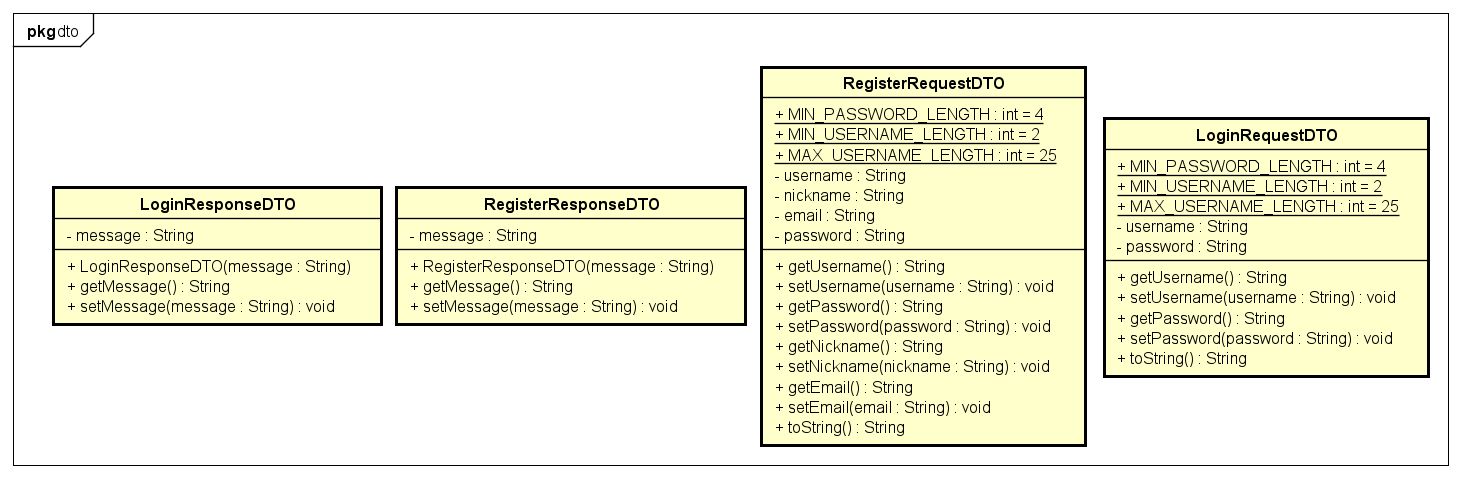
\includegraphics[width=\textwidth]{dijagrami/UML dtoovi.png}
				\caption{Dijagram razreda - dio DTO-ovi}
			\end{figure}
		
		    \begin{figure}[H]
		    	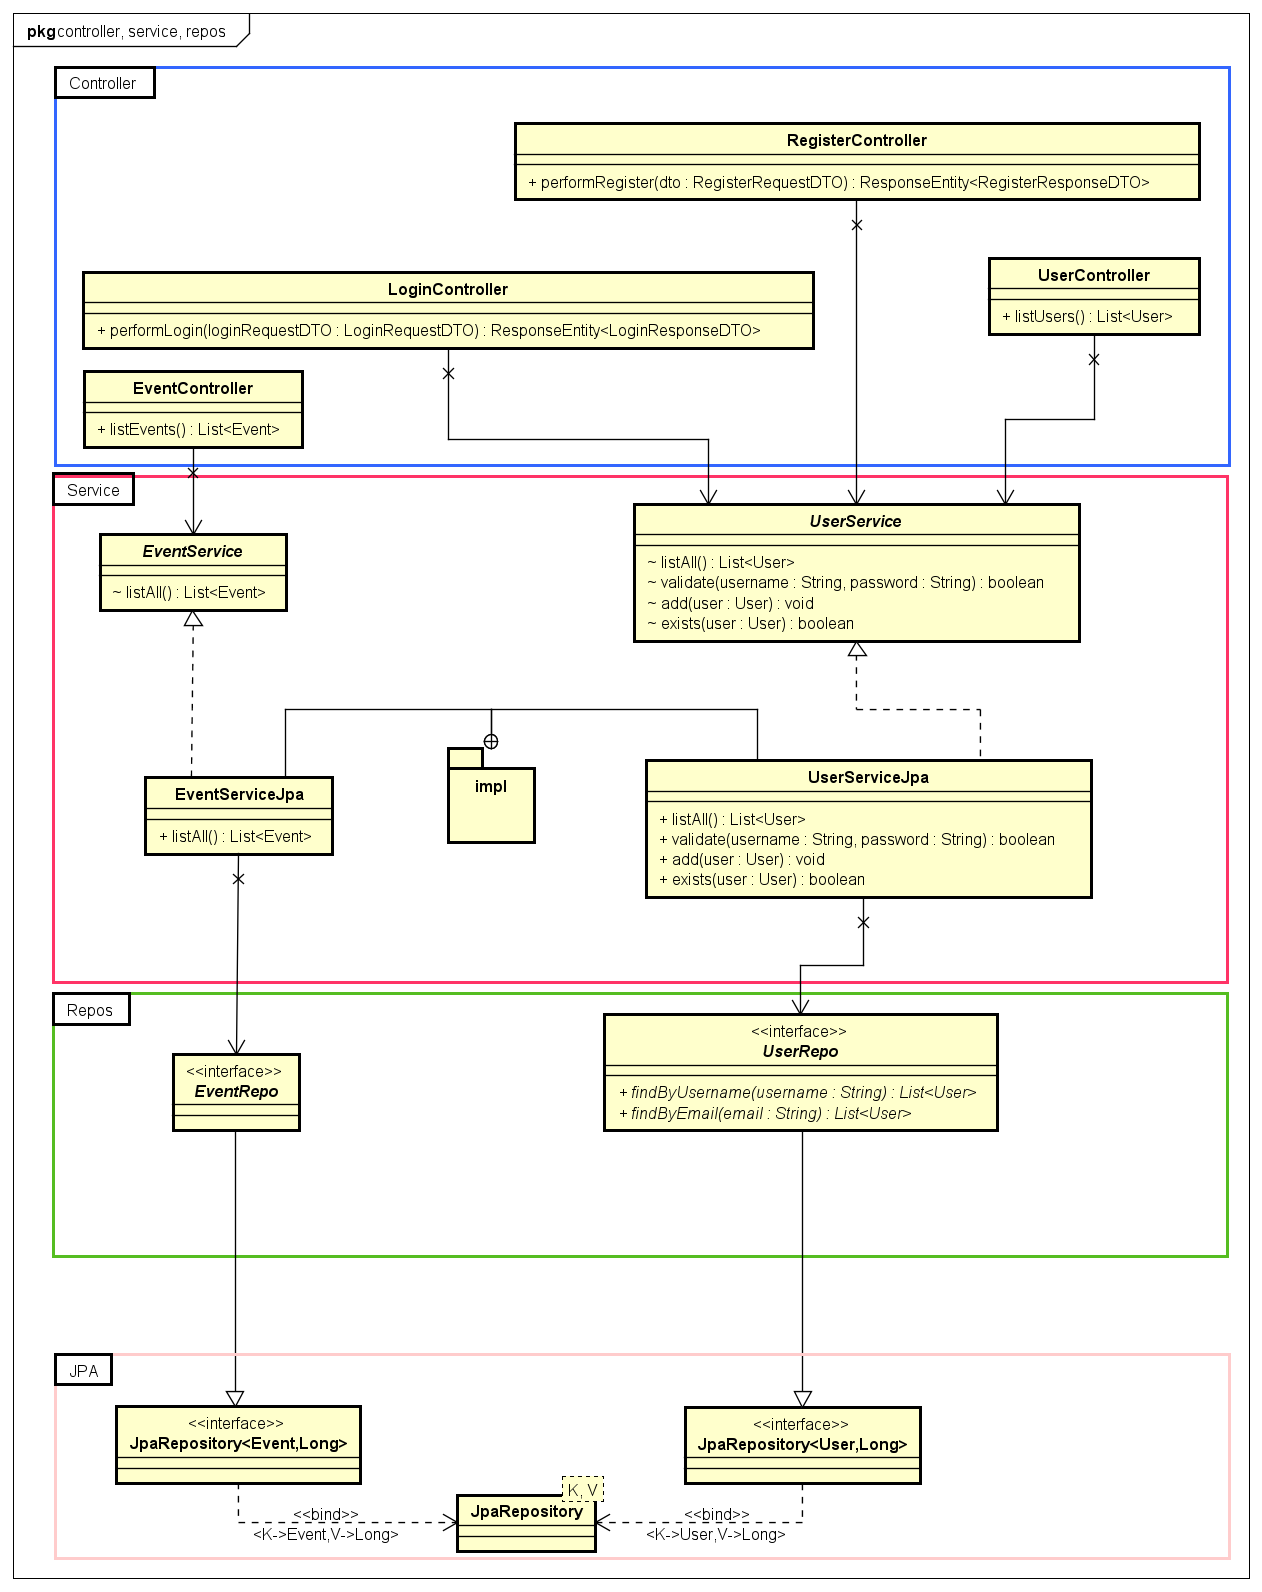
\includegraphics[width=\textwidth]{dijagrami/UML kontroleri, servisi, repozitoriji.png}
		    	\caption{Dijagram razreda - dio Kontroleri, servisi i repozitoriji}
		    \end{figure}
			
			\begin{figure}[H]
				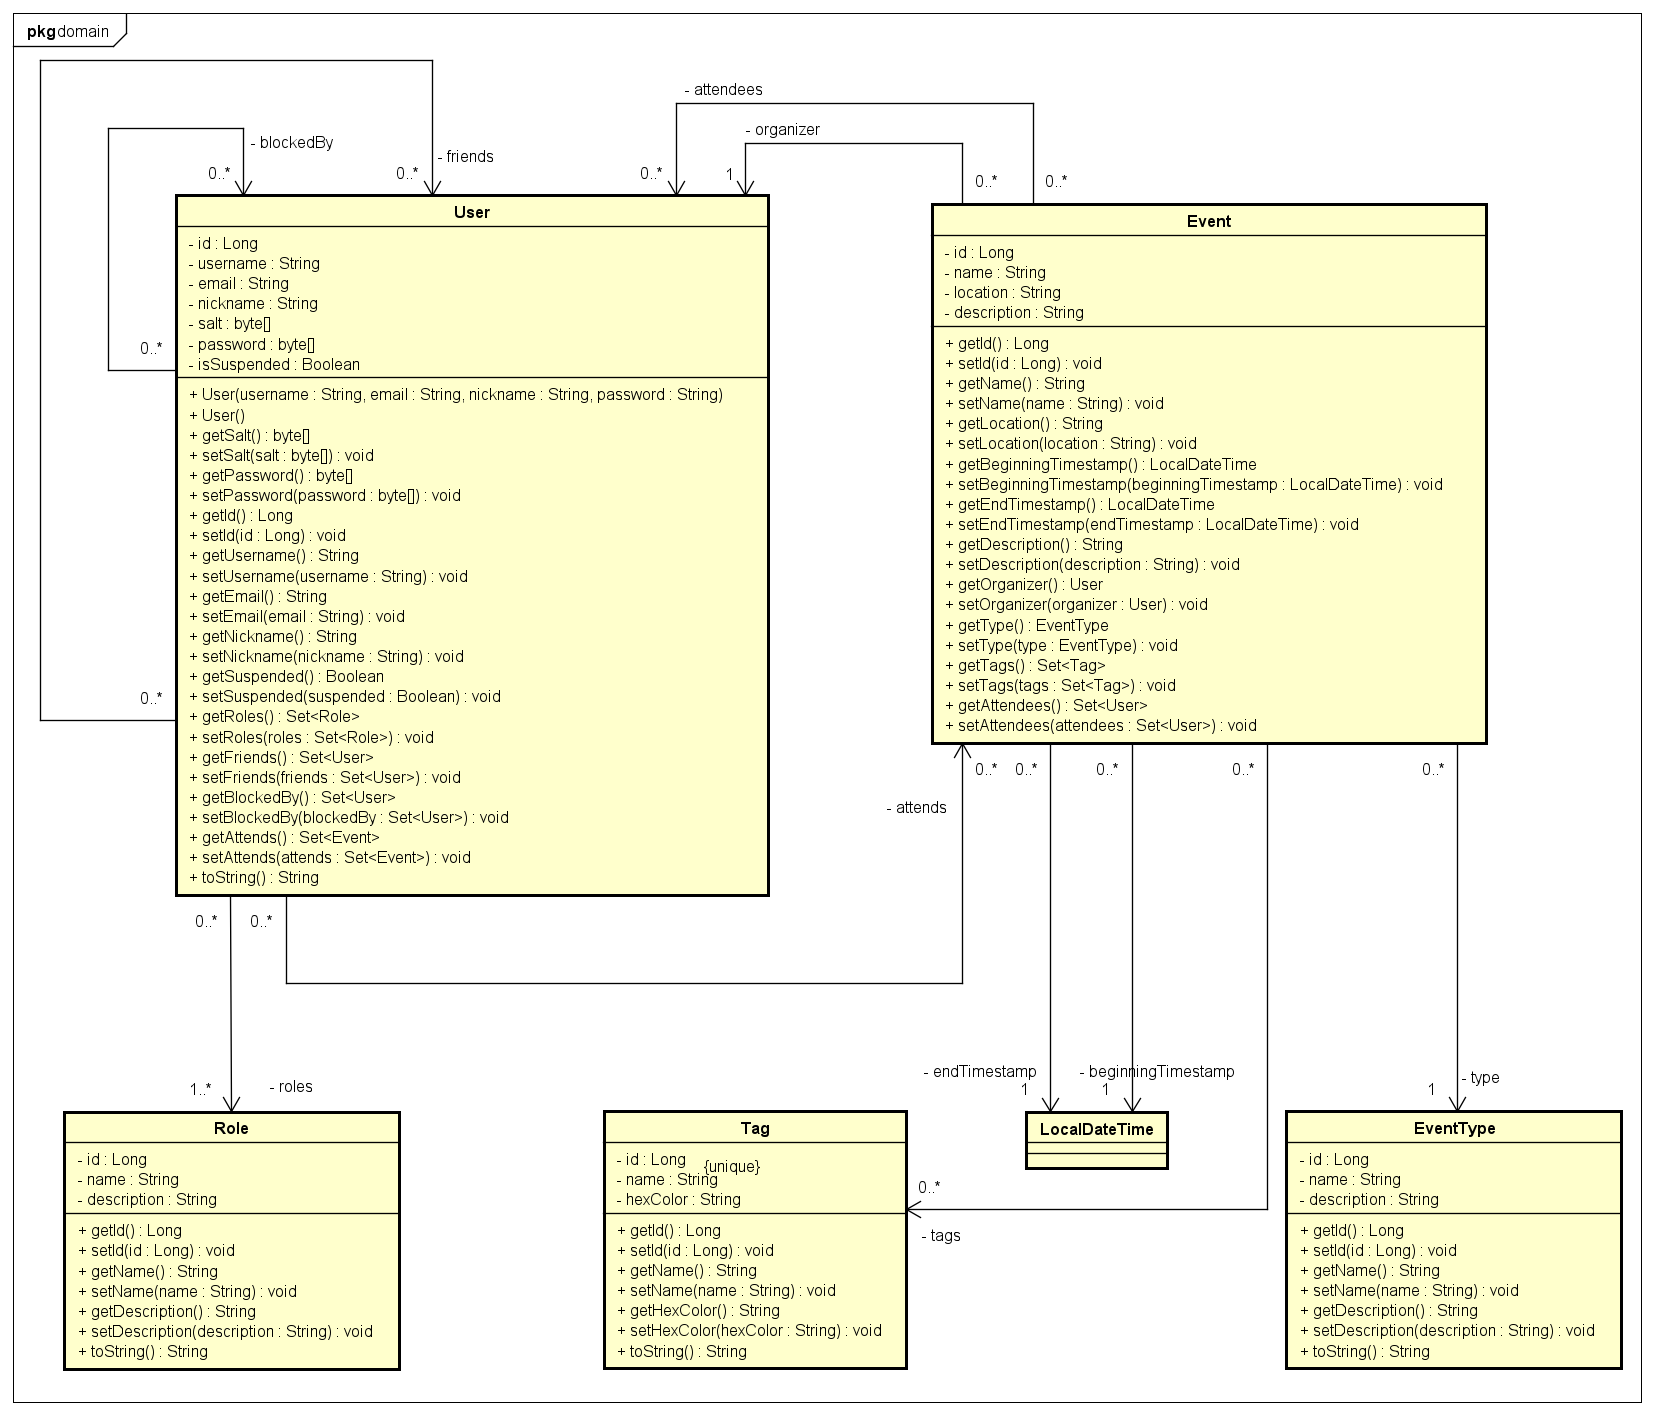
\includegraphics[width=\textwidth]{dijagrami/UML modeli.png}
				\caption{Dijagram razreda - dio Modeli}
			\end{figure}
		
			\eject
		
			
				\textbf{\textit{dio 2. revizije}}\\			
			
				\textit{Prilikom druge predaje projekta dijagram razreda i opisi moraju odgovarati stvarnom stanju implementacije}
			
			
			
				\eject
		
			\section{Dijagram stanja}
			
			
				\textbf{\textit{dio 2. revizije}}\\
			
				\textit{Potrebno je priložiti dijagram stanja i opisati ga. Dovoljan je jedan dijagram stanja koji prikazuje \textbf{značajan dio funkcionalnosti} sustava. Na primjer, stanja korisničkog sučelja i tijek korištenja neke ključne funkcionalnosti jesu značajan dio sustava, a registracija i prijava nisu. }
			
			
				\eject 
		
			\section{Dijagram aktivnosti}
			
				\textbf{\textit{dio 2. revizije}}\\
			
			 	\textit{Potrebno je priložiti dijagram aktivnosti s pripadajućim opisom. Dijagram aktivnosti treba prikazivati značajan dio sustava.}
			
				\eject
			\section{Dijagram komponenti}
		
				\textbf{\textit{dio 2. revizije}}\\
		
			 	\textit{Potrebno je priložiti dijagram komponenti s pripadajućim opisom. Dijagram komponenti treba prikazivati strukturu cijele aplikacije.}